\documentclass[tikz,border=3pt]{standalone}
\usepackage{amsmath,bm,xcolor}
\usetikzlibrary{arrows.meta}
\begin{document}
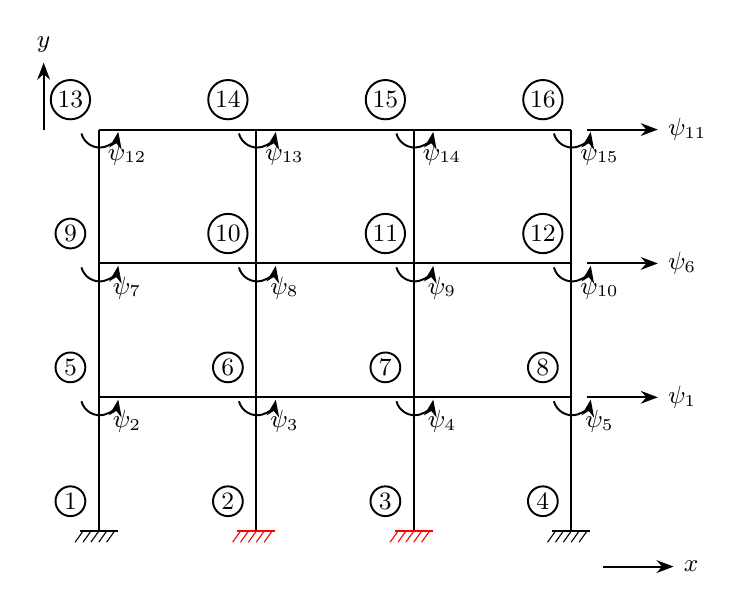
\begin{tikzpicture}[>=Stealth,every node/.style={font=\fontsize{9}{11}\selectfont},line width=.7pt]
\draw[] (0,0)--(0,5.1);
\draw[black] (-0.24,0)--(0.24,0);
\draw[black,line width=.4pt] (-0.2,0)--(-0.3,-0.14);
\draw[black,line width=.4pt] (-0.1,0)--(-0.2,-0.14);
\draw[black,line width=.4pt] (0,0)--(-0.1,-0.14);
\draw[black,line width=.4pt] (0.1,0)--(0,-0.14);
\draw[black,line width=.4pt] (0.2,0)--(0.1,-0.14);
\draw[] (2,0)--(2,5.1);
\draw[red] (1.76,0)--(2.24,0);
\draw[red,line width=.4pt] (1.8,0)--(1.7,-0.14);
\draw[red,line width=.4pt] (1.9,0)--(1.8,-0.14);
\draw[red,line width=.4pt] (2,0)--(1.9,-0.14);
\draw[red,line width=.4pt] (2.1,0)--(2,-0.14);
\draw[red,line width=.4pt] (2.2,0)--(2.1,-0.14);
\draw[] (4,0)--(4,5.1);
\draw[red] (3.76,0)--(4.24,0);
\draw[red,line width=.4pt] (3.8,0)--(3.7,-0.14);
\draw[red,line width=.4pt] (3.9,0)--(3.8,-0.14);
\draw[red,line width=.4pt] (4,0)--(3.9,-0.14);
\draw[red,line width=.4pt] (4.1,0)--(4,-0.14);
\draw[red,line width=.4pt] (4.2,0)--(4.1,-0.14);
\draw[] (6,0)--(6,5.1);
\draw[black] (5.76,0)--(6.24,0);
\draw[black,line width=.4pt] (5.8,0)--(5.7,-0.14);
\draw[black,line width=.4pt] (5.9,0)--(5.8,-0.14);
\draw[black,line width=.4pt] (6,0)--(5.9,-0.14);
\draw[black,line width=.4pt] (6.1,0)--(6,-0.14);
\draw[black,line width=.4pt] (6.2,0)--(6.1,-0.14);
\node[circle,draw,inner sep=1.2pt] at (-0.36,0.38) {1};
\node[circle,draw,inner sep=1.2pt] at (1.64,0.38) {2};
\node[circle,draw,inner sep=1.2pt] at (3.64,0.38) {3};
\node[circle,draw,inner sep=1.2pt] at (5.64,0.38) {4};
\draw[] (0,1.7)--(6,1.7);
\node[circle,draw,inner sep=1.2pt] at (-0.36,2.08) {5};
\draw[->] (-0.22,1.65) arc (195:350:.24);
\node[] at (0.36,1.39) {$\psi_{2}$};
\node[circle,draw,inner sep=1.2pt] at (1.64,2.08) {6};
\draw[->] (1.78,1.65) arc (195:350:.24);
\node[] at (2.36,1.39) {$\psi_{3}$};
\node[circle,draw,inner sep=1.2pt] at (3.64,2.08) {7};
\draw[->] (3.78,1.65) arc (195:350:.24);
\node[] at (4.36,1.39) {$\psi_{4}$};
\node[circle,draw,inner sep=1.2pt] at (5.64,2.08) {8};
\draw[->] (5.78,1.65) arc (195:350:.24);
\node[] at (6.36,1.39) {$\psi_{5}$};
\draw[->] (6.2,1.7)--(7.1,1.7) node[right] {$\psi_{1}$};
\draw[] (0,3.4)--(6,3.4);
\node[circle,draw,inner sep=1.2pt] at (-0.36,3.78) {9};
\draw[->] (-0.22,3.35) arc (195:350:.24);
\node[] at (0.36,3.09) {$\psi_{7}$};
\node[circle,draw,inner sep=1.2pt] at (1.64,3.78) {10};
\draw[->] (1.78,3.35) arc (195:350:.24);
\node[] at (2.36,3.09) {$\psi_{8}$};
\node[circle,draw,inner sep=1.2pt] at (3.64,3.78) {11};
\draw[->] (3.78,3.35) arc (195:350:.24);
\node[] at (4.36,3.09) {$\psi_{9}$};
\node[circle,draw,inner sep=1.2pt] at (5.64,3.78) {12};
\draw[->] (5.78,3.35) arc (195:350:.24);
\node[] at (6.36,3.09) {$\psi_{10}$};
\draw[->] (6.2,3.4)--(7.1,3.4) node[right] {$\psi_{6}$};
\draw[] (0,5.1)--(6,5.1);
\node[circle,draw,inner sep=1.2pt] at (-0.36,5.48) {13};
\draw[->] (-0.22,5.05) arc (195:350:.24);
\node[] at (0.36,4.79) {$\psi_{12}$};
\node[circle,draw,inner sep=1.2pt] at (1.64,5.48) {14};
\draw[->] (1.78,5.05) arc (195:350:.24);
\node[] at (2.36,4.79) {$\psi_{13}$};
\node[circle,draw,inner sep=1.2pt] at (3.64,5.48) {15};
\draw[->] (3.78,5.05) arc (195:350:.24);
\node[] at (4.36,4.79) {$\psi_{14}$};
\node[circle,draw,inner sep=1.2pt] at (5.64,5.48) {16};
\draw[->] (5.78,5.05) arc (195:350:.24);
\node[] at (6.36,4.79) {$\psi_{15}$};
\draw[->] (6.2,5.1)--(7.1,5.1) node[right] {$\psi_{11}$};
\draw[->] (-.7,5.1)--(-.7,5.95) node[above] {$y$};
\draw[->] (6.4,-.45)--(7.3,-.45) node[right] {$x$};
\end{tikzpicture}
\end{document}
